\begin{figure}
    \centering
    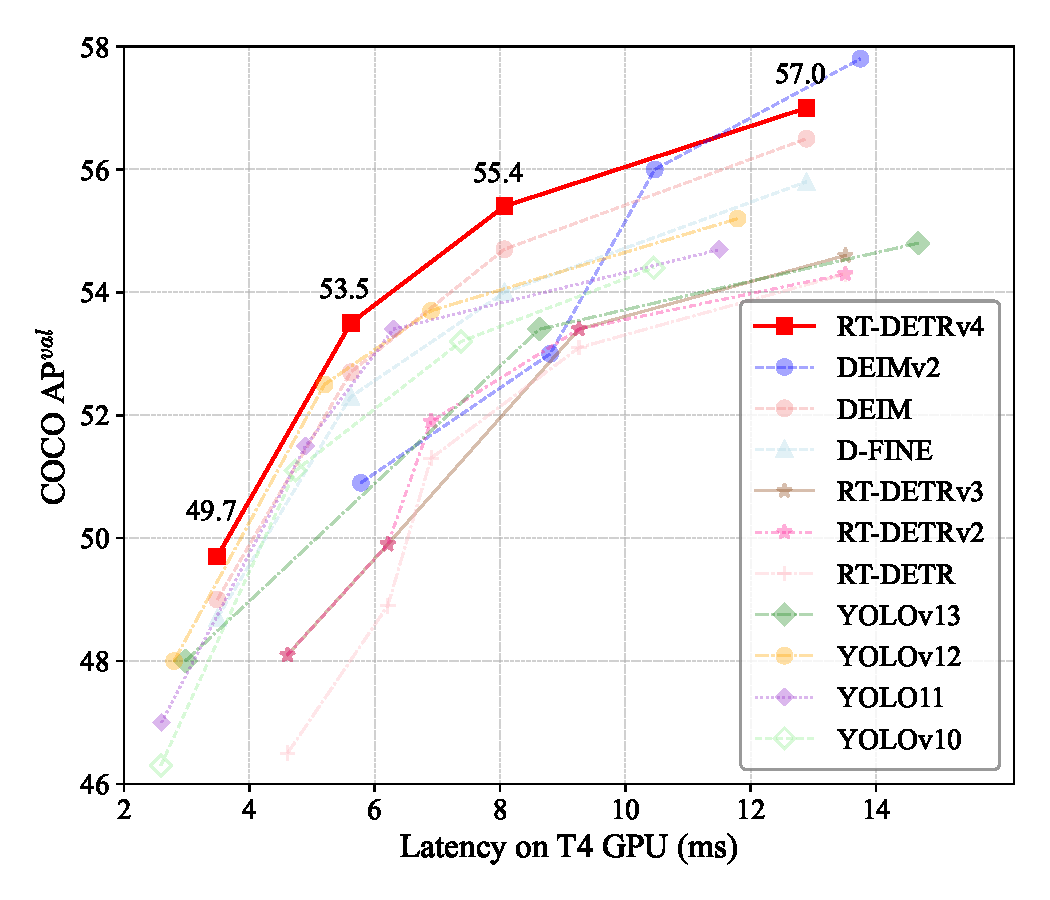
\includegraphics[width=1\linewidth]{figures/coco_ap_latency.pdf}
    \captionof{figure}{\textbf{Compared with existing advanced real-time object detectors on COCO \cite{lin2014microsoft}}. Our RT-DETRv4 models  achieve state-of-the-art performance.}
    \label{fig:coco_ap_latency}
\end{figure}

\section{Introduction}
\label{sec:intro}
Real-time object detection stands as a fundamental task in computer vision, which underpins numerous interactive and safety-critical applications that demand instant perception and decision making, such as autonomous driving~\cite{chen2024end}, embodied intelligence~\cite{liu2025embodied}, and human–computer interaction~\cite{kirillov2023segment}. 
Over the past decade, remarkable progress has been driven by increasingly efficient network architectures and end-to-end learning frameworks. 
In particular, two representative series, YOLO~\cite{redmon2016you} and DETR~\cite{carion2020end}, have profoundly influenced the evolution of object detection paradigms. The YOLO family emphasizes rapid one-stage detection achieving high inference speed and practical deployment efficiency, and the DETR series has reshaped the detection paradigm through its unified modeling of object queries and set-based prediction.
Among its variants, RT-DETR~\cite{zhao2024detrs} marked a milestone as the first real-time DETR, introducing the DETR family to the real-time community by outperforming YOLO models in both speed and accuracy.

Despite the remarkable progress, a long-standing challenge remains: the inherent trade-off between designing lightweight models to achieve high inference speed and employing complex architectures to improve feature representation.
To meet real-time constraints, detectors typically adopt lightweight backbones and carefully designed computational modules, which inevitably reduce their ability to capture high-level semantics and lead to a semantic bottleneck.
This limitation not only hinders further performance improvement but also increases the difficulty of practical on-device deployment.

In this paper, inspired by the rapid advances in Vision Foundation Models (VFMs)~\cite{simeoni2025dinov3,he2022masked}, we propose a cost-effective and highly adaptable distillation framework that leverages the powerful representational capacity of VFMs to enhance lightweight object detectors.
By transferring the rich semantics of VFMs to real-time detectors during training while keeping the detector architecture unchanged during inference, our method enables significant enhancement without introducing any additional inference or deployment cost.
This advantage is particularly important for practical real-time detection applications.

However, achieving stable and task-aligned semantic transfer is challenging because of the large architectural and learning objective disparities between VFMs and resource-constrained detectors.
To address this issue, we first introduce a Deep Semantic Injector (DSI) module that enables the integration of high-level representations from VFMs into the deep layers of the detector.
To ensure stable and efficient optimization, we further design a Gradient-guided Adaptive Modulation (GAM) strategy that dynamically adjusts the strength of semantic injection based on gradient norm ratios, thereby harmonizing the learning of semantic transfer and detection objectives.

Extensive experiments demonstrate that the proposed framework achieves consistent and significant performance improvements over advanced DETR-based detectors without increasing inference or deployment overhead, underscoring its effectiveness.
In summary, our main contributions are as follows:
\begin{itemize}
\item We propose a cost-effective and highly adaptable distillation framework that leverages the evolving capabilities of VFMs to painlessly enhance real-time detectors, providing a scalable pathway for transferring foundation-level semantics to lightweight architectures.
\item We propose the Deep Semantic Injector (DSI) and Gradient-guided Adaptive Modulation (GAM), which enable stable and task-aligned semantic transfer between VFMs and detectors with significantly different architectures and learning objectives.
\item We establish a new family of models, \ourmethod-S/M/L/X, achieving $49.7 / 53.5 / 55.4 / 57.0$ AP scores on COCO~\cite{lin2014microsoft} at $273 / 169 / 124 / 78$ FPS, setting a new SOTA on COCO dataset.
\end{itemize}